\documentclass[
    reprint, 
    aps,
    preprintnumbers,
    twocolumn,
    prb,
    superscriptaddress
]{revtex4-2}


%=======================
% Packages:
%=======================

\usepackage[utf8]{inputenc}
\usepackage{booktabs}
\usepackage[multiple]{footmisc}
\usepackage{lipsum}
\usepackage{rotating}
\usepackage{perpage}
\usepackage{chronology}
\usepackage{lipsum}
\usepackage{amssymb}
\usepackage{amsbsy}
\usepackage{amsmath}
\usepackage{tikz}
\usepackage[T1]{fontenc}
\usepackage{etoolbox}
\usepackage{graphics}
\usepackage{abraces}
\makeatletter
\let\unit\relax % otherwise there are package conflicts with siunitx
\makeatother
\usepackage{siunitx}
\usepackage{hyperref}
%\usepackage{float}
\usepackage{multirow}
\usepackage{mathtools}
\usepackage{bm}
\usepackage{url}
\usepackage{physics}
\usepackage{hyperref}
\usepackage{bbm}
\usepackage{color}
\usepackage{placeins}
\usepackage[normalem]{ulem}
\usepackage{mhchem}


%=======================
% New Commands:
%=======================

\newcommand{\vk}{\vec{k}}
\newcommand{\vQ}{\vec{Q}}
\newcommand{\up}{\uparrow}
\newcommand{\down}{\downarrow}
\newcommand{\kplusQ}{\vk+\vQ}
\newcommand{\kminusQ}{-\vk-\vQ}

\newcommand{\ddt}{\frac{\mathrm{d}}{\mathrm{d}t}}
\newcommand{\dgamma}{\mathrm{d}\gamma}

\begin{document} 

% Preliminary title
\title{Collective excitations in the 2- and 3-dimensional extended Hubbard model}

%=======================
% Authors:
%=======================

\author{Joshua Alth\"user}\email{joshua.althueser@tu-dortmund.de}
\affiliation{Condensed Matter Theory, TU Dortmund University,
Otto-Hahn Stra\ss{}e 4, 44221 Dortmund, Germany}

\author{G\"otz S.~Uhrig}
\email{goetz.uhrig@tu-dortmund.de}
\affiliation{Condensed Matter Theory, TU Dortmund University,
Otto-Hahn Stra\ss{}e 4, 44221 Dortmund, Germany}

\date{\today}

%%%%%%%%%%%%%%%%%%%%%%%%%%%%%%%%%%%%%%%%%%%%%%%%%%%%%%%%%%%%%%%%%%%%%%%%%%%%%%%%%%%%%%%%%%%%%%%%%%%%%%%%%%%%%%%%%%%%%
%%%%%%%%%%%%%%%%%%%%%%%%%%%%%%%%%%%%%%%%%%%%%%%%%%%%%%%%%%%%%%%%%%%%%%%%%%%%%%%%%%%%%%%%%%%%%%%%%%%%%%%%%%%%%%%%%%%%%
%%%%%                                                  Abstract                                                 %%%%%
%%%%%%%%%%%%%%%%%%%%%%%%%%%%%%%%%%%%%%%%%%%%%%%%%%%%%%%%%%%%%%%%%%%%%%%%%%%%%%%%%%%%%%%%%%%%%%%%%%%%%%%%%%%%%%%%%%%%%
%%%%%%%%%%%%%%%%%%%%%%%%%%%%%%%%%%%%%%%%%%%%%%%%%%%%%%%%%%%%%%%%%%%%%%%%%%%%%%%%%%%%%%%%%%%%%%%%%%%%%%%%%%%%%%%%%%%%%
\begin{abstract}
    We investigate the superconducting (SC), charge-density wave (CDW), and antiferromagnetic (AFM) phases 
    in the extended Hubbard model at zero temperature and half-filling.
    We employ the iterated equations of motion approach \cite{Kalthoff17,bleicker18} to compute the two-particle Green's functions and
    by extension, the corresponding spectral densities.
    This renders a comprehensive analysis of the behaviour of collective excitations possible
    as the model's parameters are changed across phase transitions.
    We identify the well-known amplitude (Higgs) and phase (Leggett) modes within the 
    superconducting phase and observe a similar excitation in the CDW phase
    which shift towards zero energy as the system approaches the phase transition to the SC phase.
    In the CDW phase, close to the phase transition to the AFM phase, we find a collective mode 
    which does not change significantly and another modes which becomes soft
    as the phase boundary is approached.
\end{abstract}

\maketitle

%%%%%%%%%%%%%%%%%%%%%%%%%%%%%%%%%%%%%%%%%%%%%%%%%%%%%%%%%%%%%%%%%%%%%%%%%%%%%%%%%%%%%%%%%%%%%%%%%%%%%%%%%%%%%%%%%%%%%
%%%%%%%%%%%%%%%%%%%%%%%%%%%%%%%%%%%%%%%%%%%%%%%%%%%%%%%%%%%%%%%%%%%%%%%%%%%%%%%%%%%%%%%%%%%%%%%%%%%%%%%%%%%%%%%%%%%%%
%%%%%                                                Introduction                                               %%%%%
%%%%%%%%%%%%%%%%%%%%%%%%%%%%%%%%%%%%%%%%%%%%%%%%%%%%%%%%%%%%%%%%%%%%%%%%%%%%%%%%%%%%%%%%%%%%%%%%%%%%%%%%%%%%%%%%%%%%%
%%%%%%%%%%%%%%%%%%%%%%%%%%%%%%%%%%%%%%%%%%%%%%%%%%%%%%%%%%%%%%%%%%%%%%%%%%%%%%%%%%%%%%%%%%%%%%%%%%%%%%%%%%%%%%%%%%%%%

\section{Introduction}\label{sec:introduction}

The Hubbard model has been studied in a plethora of previous studies. 
Early studies proved the existence of eigenstates to the Hubbard Hamiltonian that exhibit off-diagonal long-range order,
encouraging the model's usage for the description of high-temperature superconductivity \cite{yang89}.
Shortly afterward, an exact $SO(4)$ symmetry was discovered,
which allows a degeneracy of superconductivity (SC) and a charge-density wave (CDW) governed by an attractive on-site interaction \cite{yang90}.
This coexistence can be argued by the existence of a particle-hole transformation on bipartite lattices, 
that maps the attractive Hubbard model exactly onto the repulsive one, exhibiting antiferromagnetism (AFM) \cite{Hirsch85}.
The previously mentioned SC and CDW phases map to different spin operators \cite{zitko15,lieb89}.
\newline
Many recent experimental and theoretical studies examined the driven systems in the hope of inducing superconductivity 
\cite{Nicoletti14,Krull14,Moor14,Casandruc15,patel16,sentef17,Buenemann17}.
Other studies, focusing on equilibrium systems, 
investigated the phases and various quantities therein of the said model including various additional interactions with and without doping 
\cite{Micnas88,Micnas88b,Micnas89,Dzierzawa92,Kostyrko92,Eriksson95,Staudt00,Onari04,Toschi05,Brackett16,Paki19,romer20,Sushchyev22}.
\newline
In this paper, we will restrict ourselves to the half-filled Hubbard model, including an additional intersite interaction, on a square and a simple cubic lattice.
\textcolor{red}{Für den 3D Fall finde ich keine Phasendiagramme des extended Hubbard models, ggf nochmal suchen...}
The 2D case already exhibits a wide range of possible phases, including CDW, AFM as well as $s$- and $d_{x^2 - y^2}$-wave superconductivity
\cite{Micnas88b,Tsuchiura95,Su01,Su04,ha11,Huang13,Jiang22}.
\newline
In this article, we will first employ a mean-field approximation to the interaction terms 
and then use the methodology from the so-called iterated equations of motion approach,
which has already seen success in the handling of interaction quenches \cite{uhrig09,hamerla13,hamerla14,bleicker18}.
Here, one commutes operators from a suitable operator basis with the Hamiltonian and adds the newly occurring terms to it.
Naturally, a truncation is necessary for most practical applications, however, the approximation becomes better the more terms are included within the basis.
The functionality of this method has been compared to the density matrix formalism and has proved to be considerably more accurate \cite{Kalthoff17}.
Additionally, we will show an explicit way to obtain various Green's functions from the aforementioned methodology.
By extension, we also obtain the spectral functions of the investigated systems and discuss the excitations found therein.
The prominent examples in the SC phase are the well-known phase (Leggett) and amplitude (Higgs) modes \cite{Cea14,Krull16,Schwarz20,Fan22}.
\newline
The remainder of this paper is organized as follows:
In \autoref{sec:model} we will introduce the model and its Hamiltonian as well our mean-field theory.
A brief overview over the iterated equations of motion approach is presented in \autoref{sec:ieom}.
Next, we show our results in \autoref{sec:results}.
Lastly, in \autoref{sec:conclusion}, we will discuss our results.
In the appendix \textcolor{red}{(or in the supplemental material?)}, we will derive and explain our methods in detail.

\section{Model and mean-field theory}\label{sec:model}

The Hamiltonian of the extended Hubbard model is given by
\begin{equation}
    \label{eqn:full_hamiltonian}
    \begin{aligned}
        H = &-t \sum_{\langle i, j \rangle, \sigma} \left( c_{i\sigma}^\dagger c_{j\sigma} + \text{h.c.} \right) 
        + \mu \sum_{i,\sigma} n_{i\sigma} \\
        &+ U \sum_{i} n_{i\uparrow} n_{i\downarrow} 
        + \frac{V}{2} \sum_{\langle i, j\rangle, \sigma} n_{i\sigma} n_{j\sigma}\,,
    \end{aligned}
\end{equation}

where $c_{i\sigma}^{(\dagger)}$ annihilates (creates) an electron with spin $\sigma$ on lattice site $i$ and $\langle i, j\rangle$ denotes the summation over next neighbours.
The parameters are the hopping amplitude $t$, the onsite interaction $U$, the intersite interaction $V$ and the chemical potential $\mu$.
Throughout this article, we will give all energy-related quantities in terms of the hopping amplitude, which we subsequently set to unity $t=1$.
Applying a Fourier transformation into $k$-space yields the single-particle dispersion 

\begin{equation}
    \epsilon_0 (\vk) = -2t \sum_{\alpha=1}^D \cos(k_\alpha)\,,\quad k_\alpha \in [-\pi, \pi)\,,
\end{equation}
with the system's dimension $D$ and the dimensionless momentum $\vk$.
The interaction terms are then mean-field decoupled. 
We follow the naming scheme of Ref. \cite{sentef17}

\begin{equation}
    \label{eqn:operators}
    \begin{aligned}
        n_{k\sigma} &:= c_{\vk\sigma}^\dagger c_{\vk\sigma}\,,      &f_k     &:= c_{-\vk\down} c_{\vk\up}\,, \\
        g_{k\sigma} &:= c_{\vk\sigma}^\dagger c_{\vk+\vQ\sigma}\,,  &\eta_k  &:= c_{-\vk-\vQ\down} c_{\vk\up}\,,
    \end{aligned}
\end{equation}

where $\vQ := (\pi, ...)$ defines the nesting vector for the CDW and AFM phases.
We use the following abbreviations to write down the mean-field parameters

\begin{subequations}
    \begin{align}
        \label{eqn:delta_cdw}
        \Delta_\text{CDW} &= \left(\frac{U}{2N} - \frac{ZV}{N}\right) \sum_{\vk\sigma} \langle g_{\vk\sigma} \rangle\,, \\
        \label{eqn:delta_afm}
        \Delta_\text{AFM} &= \frac{U}{2N} \sum_{\vk} \left( \langle g_{k\uparrow} \rangle - \langle g_{\vk\downarrow} \rangle \right)\,, \\
        \Delta_\text{SC} &= \frac{U}{N} \sum_{\vk} \langle f_{\vk} \rangle\,, \\
        \Delta_\eta &= \frac{U}{N} \sum_{\vk} \langle \eta_{\vk} \rangle\,, \\
        \Delta_n &= \frac{V}{N} \sum_{\vk,\sigma} \sum_{\alpha=1}^D \cos k_\alpha \langle n_{\vk\sigma} \rangle\,,
    \end{align}
\end{subequations}

where $Z$ denotes the coordination number of the lattice.
The last parameter, $\Delta_n$, renormalizes the hoping term to

\begin{equation}
    \epsilon( \vk ) := -(2 + \Delta_n) \sum_{\alpha=1}^D \cos(k_\alpha)\,.
\end{equation}

In total, we obtain the mean-field Hamiltonian in spinor representation as

\begin{equation}
    \label{eqn:mf_hamiltonian}
    H_\text{MF} = \sum_{\vk} \Psi^\dagger (\vk) h(\vk) \Psi (\vk)\,,
\end{equation}

with the spinors
\begin{equation}
    \Psi^\dagger (\vk) := \left( c_{\vk\up}^\dagger\,, c_{\kplusQ\up}^\dagger\,, c_{-\vk\down}\,, c_{\kminusQ\down} \right)
\end{equation}

and 

\begin{widetext}
\begin{equation}
    h(\vk) := \begin{pmatrix}
        \epsilon (\vk) & \Delta_\text{CDW}^* - \Delta_\text{AFM}^* & \Delta_\text{SC} & \Delta_\eta \\
        \Delta_\text{CDW} - \Delta_\text{AFM} & \epsilon (\vk + \vQ) & \Delta_\eta & \Delta_\text{SC} \\
        \Delta_\text{SC}^* & \Delta_\eta^* & - \epsilon (-\vk) & - \Delta_\text{CDW} - \Delta_\text{AFM} \\
        \Delta_\eta^* & \Delta_\text{SC}^* & - \Delta_\text{CDW}^* - \Delta_\text{AFM}^* & - \epsilon (-\vk - \vQ)\,.
        \end{pmatrix}
\end{equation}
\end{widetext}

\begin{figure}
    \centering
    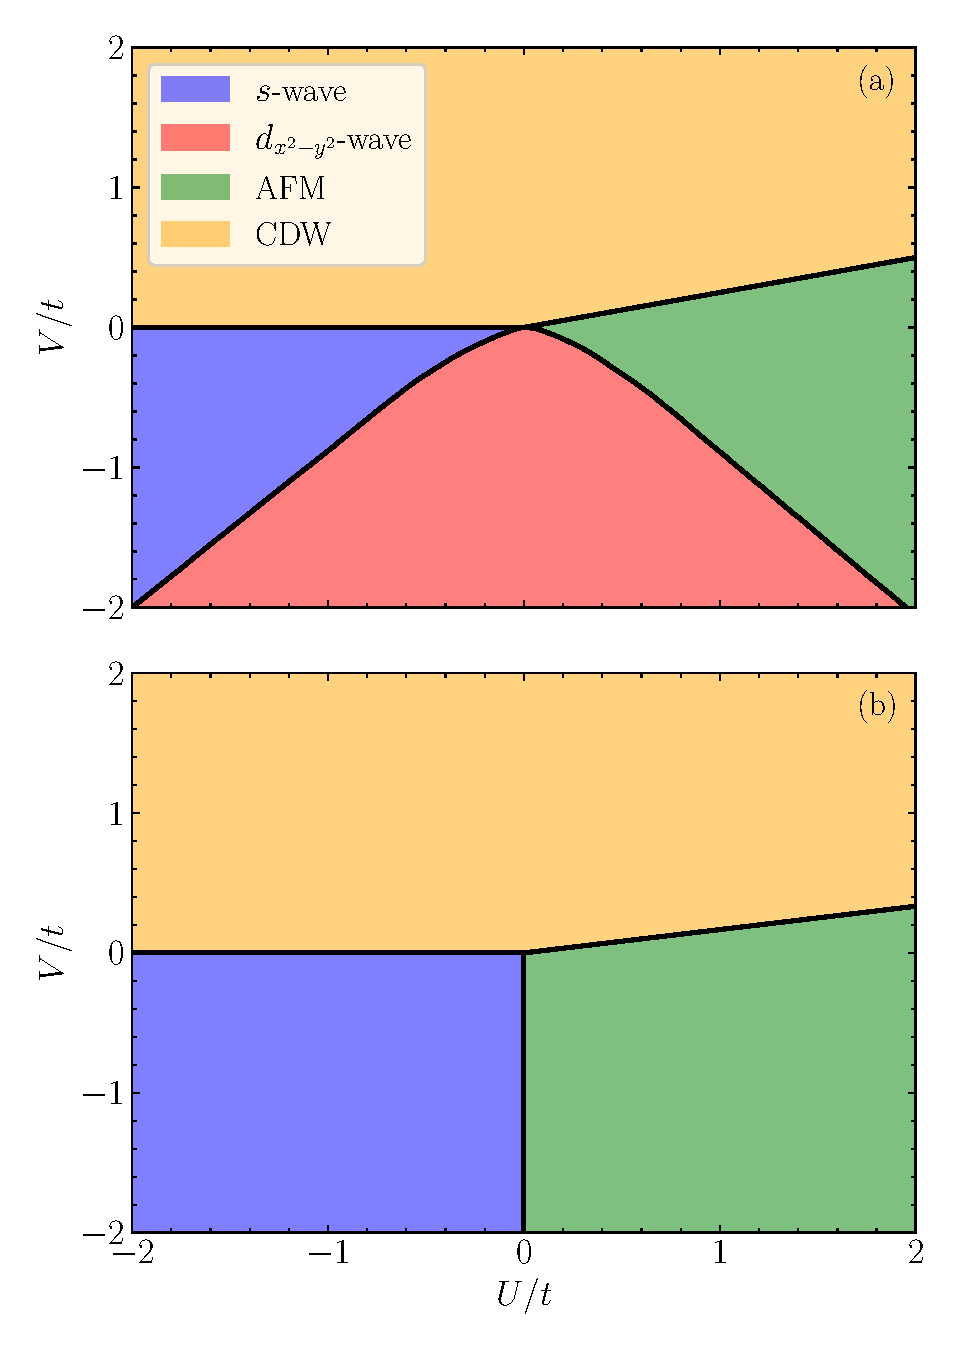
\includegraphics[width=.48\textwidth]{plots/phase_diagram.pdf}
    \caption{The phase diagram obtained for the extended Hubbard model on (a) a square lattice and (b) a simple cubic lattice using a mean-field approximation at temperature $T=0$.
    The CDW-AFM boundary lies at $U = ZV$, where $Z$ is the coordination number. For $U<0$ and $V=0$, there is a coexistence of CDW and $s$-wave SC.
    The boundary for the $d_{x^2 - y^2}$-wave SC for the square lattice has been taken from Ref. \cite{Micnas88b}, as it is not accessible using our formalism.}
    \label{fig:phase_diagram}
\end{figure}

Now, the entire Hamiltonian and thus all expectation values only depend on
\begin{equation}
    \hat{\gamma}(\vk) := \sum_{\alpha=1}^D \cos(k_\alpha)\,,
\end{equation}
i.e. for any operator $O$ the following relation holds 
\begin{equation}
    \label{eqn:equal_expecs}
    \langle O_{\vk} \rangle = \langle O_{\vk'} \rangle =: \langle O_{\gamma} \rangle\,,
\end{equation}
if $\hat{\gamma}(\vk) = \hat{\gamma}(\vk')$.
This allows us to replace the momentum sums with energy integrals using the bare density of states
\begin{equation}
    \rho(\gamma) := \frac{1}{N} \sum_{\vk} \delta \left(\gamma - \hat{\gamma} (\vk) \right)\,.
\end{equation}
As an example, consider 
\begin{equation}
    \Delta_\text{SC} = \frac{U}{2N} \int \dgamma \rho(\gamma) \langle f_{\gamma} \rangle\,.
\end{equation}
We will be using the exact densities of states for the square and the simple cubic lattice found in Ref. \cite{Hanisch97}.
Solving the mean-field equations iteratively, one obtains the groundstate phase diagram at temperature $T=0$ as shown in \autoref{fig:phase_diagram}.
Note, that the $d_{x^2 - y^2}$-superconducting state, which has been confirmed for the square lattice \cite{Micnas88b,Huang13}, cannot be described by our method. 
This is due to our restriction to terms that are proportional to $\hat{\gamma}(\vk)$.
\newline
The CDW-AFM boundary is located at $U = ZV$, where $Z$ is the coordination.
This holds for both the square lattice ($Z=4$) and the simple cubic lattice ($Z=6$) and can be seen by comparing \eqref{eqn:delta_cdw} and \eqref{eqn:delta_afm}:
Crossing the aforementioned line, changes which one of the two prefactors is larger.


%%%%%%%%%%%%%%%%%%%%%%%%%%%%%%%%%%%%%%%%%%%%%%%%%%%%%%%%%%%%%%%%%%%%%%%%%%%%%%%%%%%%%%%%%%%%%%%%%%%%%%%%%%%%%%%%%%%%%
%%%%%%%%%%%%%%%%%%%%%%%%%%%%%%%%%%%%%%%%%%%%%%%%%%%%%%%%%%%%%%%%%%%%%%%%%%%%%%%%%%%%%%%%%%%%%%%%%%%%%%%%%%%%%%%%%%%%%
%%%%%                                                  Methods                                                  %%%%%
%%%%%%%%%%%%%%%%%%%%%%%%%%%%%%%%%%%%%%%%%%%%%%%%%%%%%%%%%%%%%%%%%%%%%%%%%%%%%%%%%%%%%%%%%%%%%%%%%%%%%%%%%%%%%%%%%%%%%
%%%%%%%%%%%%%%%%%%%%%%%%%%%%%%%%%%%%%%%%%%%%%%%%%%%%%%%%%%%%%%%%%%%%%%%%%%%%%%%%%%%%%%%%%%%%%%%%%%%%%%%%%%%%%%%%%%%%%

\section{Iterated equations of motion and Green's functions}\label{sec:ieom}

To investigate the collective modes, we employ the iterated equations of motion approach \cite{uhrig09,hamerla13,hamerla14,bleicker18}.
We will present the general ideas briefly here and direct the interested reader to the appendix \textcolor{red}{!REF!} for a detailed explanation and derivation.
\newline
We start with some operator basis $\mathcal{B}$ that is complete with respect to commutation with a Hamiltonian $H$, 
i.e. any commutator $[H, A]$ for any $A \in \mathcal{B}$ can be represented by linear combinations of operators in $\mathcal{B}$.
We can then express any time-depend operator from this basis as

\begin{equation}
    a(t) = \sum_j c_j(t) A_j\,,
\end{equation}

where $c_j(t)$ captures the entire time dependence. 
Plugging this into the Heisenberg equation of motion and applying an operator scalar product $(A_i|\cdot)$ to both sides of the equation yields

\begin{equation}
    \label{eqn:heisenberg}
    \begin{aligned}
        \ddt a(t) = \sum_j \ddt c_j(t) A_j &= i \sum_j c_j(t) [H, A_j] \\
        \Rightarrow \sum_j \underbrace{(A_i | A_j)}_{:=\mathcal{N_{ij}}} \ddt c_j(t) &= i \sum_j \underbrace{(A_i | [H, A_j])}_{:=\mathcal{M_{ij}}} c_j(t) \\
        \Rightarrow \mathcal{N} \ddt \vec{c}(t) &= i \mathcal{M} \vec{c}(t)\,.
    \end{aligned}
\end{equation}

The matrices $\mathcal{N}$ and $\mathcal{M}$ contain all the dynamics and energetic properties of the system but have the significant advantage of being simple matrices rather than operators acting on an enormous Hilbert space.
\newline
However, most Hamiltonians do not allow any such operator basis to exist. 
Therefore, one repeats this commutation process and includes the occurring terms within a bigger basis,
hoping to get better results as the basis size increases.

In this article, we will be using the operator pseudo scalar product

\begin{equation}
\label{eqn:scalar_product}
    (A | B) := \langle [A^\dagger, B] \rangle\,,
\end{equation}

where the expectation values are taken with respect to the thermal equilibrium of the mean-field Hamiltonian \eqref{eqn:mf_hamiltonian}.
Nevertheless, we will compute $\mathcal{M}$ using the full Hubbard Hamiltonian \eqref{eqn:full_hamiltonian} enabling us to capture collective behaviour rather than the one particle dynamics given by the mean-field approximation.
\newline
This choice enables us to write down matrix-valued Fourier-transformed Green's functions in terms of the aforementioned matrices

\begin{equation}
    \label{eqn:green_function}
    \mathcal{G}(z = \omega + i0^+) = \mathcal{N} \frac{1}{-z \mathcal{N} - \mathcal{M}} \mathcal{N} := -\mathcal{N} \mathcal{R}(z) \mathcal{N}\,,
\end{equation}

where we defined the resolvent

\begin{equation}
    \label{eqn:resolvent}
    \mathcal{R}(z) := \frac{1}{z \mathcal{N} + \mathcal{M}}\,.
\end{equation}

Here, the different matrix elements correspond to various Green's functions, depending on the operator basis.
For instance, assume the operator in the basis is $f_{\vk}$, then the top left element of $\mathcal{G}$ is the Green's function 

\begin{equation}
    \mathcal{G}_{00}(z = \omega +i0^+) =  G(z) = -i \int_0^{\infty} \langle [f_{\vk}(t), f_{\vk}^\dagger(0)] \rangle e^{izt} \mathrm{d}t\,.
\end{equation}

For a detailed derivation of this statement, we refer the reader to the appendix \textcolor{red}{!REF!}.

Our operator basis consists of operators of the type

\begin{equation}
    A_\gamma := \frac{1}{\sqrt{N}} \sum_{\vk} \delta (\gamma - \hat{\gamma}( \vk )) A_{\vk}\,,
\end{equation}

where $A_{\vk}$ represents each type of operator in \eqref{eqn:operators} and their Hermitian conjugates.
Different indices are taken as additional basis operators, e.g. $n_{\vk \up}$ and $n_{\vk \down}$ are taken into the basis separately.
We then order these operators in a way reminiscent of the $x$- and $p$-terms in the harmonic oscillator, i.e.

\begin{equation}
    X_i := A_i + A_i^\dagger\,,\quad P_i := A_i - A_i^\dagger\,.
\end{equation}

Our basis is then $\mathcal{B}_{XP} := {X_i, P_i}$.
If some operators would be 0 ($P_i$ for any $n$-type term) or duplicates (certain $X_i$ for $g$-type terms), we omit them.
\newline
Due to this choice of basis, the matrices occurring in \eqref{eqn:heisenberg} have a special block structure

\begin{equation}
    \mathcal{M} = \begin{pmatrix}
        \mathcal{K}_+ & \kappa \\ \kappa^\dagger & \mathcal{K}_-
    \end{pmatrix}\,,\quad \mathcal{N} = \begin{pmatrix}
        \Lambda_+ & \mathcal{L} \\ \mathcal{L}^\dagger & \Lambda_-
    \end{pmatrix}\,,
\end{equation}

where $\Im [\mathcal{K}_\pm] = \Re [\kappa] = 0$ and $\Re [\Lambda_\pm] = \Im [\mathcal{L}] = 0$.
Furthermore, if all occurring expectation values are real, both matrices have large empty blocks.
This condition is fulfilled for all cases investigated in this article.
Additionally, we can utilize this block structure to rewrite \eqref{eqn:resolvent} to

\begin{equation}
    \mathcal{R}(z) \vert_X = - \check{N}^{-1/2} \frac{1}{z^2 - \underbrace{\check{N}^{-1/2} \mathcal{K}_+ \check{N}^{-1/2}}_{:= \check{M}}} \check{N}^{-1/2}\,,
\end{equation}

where $\vert_X$ denotes the block corresponding to the $X$-terms in the basis and $\check{N} := \mathcal{L} \mathcal{K}_-^{-1} \mathcal{L}^\dagger$.
An analogous form can be found for the $P$-block.

Now, the task at hand is finding the inverse $1/(z^2 - \check{M})$ for all $z$.
This can be achieved using a Lanczos tridiagonalization and subsequently a continued fraction expansion in the form of

\begin{widetext}
\begin{equation}
    \left( z^2 - \begin{pmatrix}
        z - a_0 & b_1 & 0 & 0 & \cdots \\
        b_1 & z - a_1 & b_2 & 0 & \cdots \\
        0 & b_2 & z - a_2 & b_3 & \cdots \\
        \vdots & \vdots & \vdots & \vdots & \ddots
    \end{pmatrix} \right)_{00}^{-1} = \dfrac{1}{z^2 - a_0 - \dfrac{b_1^2}{z^2 - a_1 - \dfrac{b_2^2}{ z^2 - a_2 - \hdots}}}\,\,
\end{equation}
\end{widetext}

where $a_i$ and $b_i$ are the Lanczos coefficients \cite{PettiforRecursion,ViswanathRecursion}.
In the single-band case, the coefficients approach the limit

\begin{equation}
    \label{eqn:inf_lanczos}
    a_\infty = \frac{\omega_+ + \omega_-}{2}\text{  and  } b_\infty = \frac{\omega_+ - \omega_-}{4}\,,
\end{equation}

where $\omega_\pm$ represent the upper and lower band edge, respectively.
This behaviour allows us to terminate the continued fraction, if the convergence is good enough, using the so-called square root terminator

\begin{equation}
    T(\omega) = \frac{1}{2b_\infty^2} \left( \omega - a_\infty \mp \sqrt{(\omega - a_\infty)^2 - 4 b_\infty^2} \right)\,,
\end{equation}

where the negative sign is to be chosen for $\omega - a_\infty > 2b_\infty$ and $|\omega - a_\infty| < 2b_\infty$ and the positive one otherwise.

%%%%%%%%%%%%%%%%%%%%%%%%%%%%%%%%%%%%%%%%%%%%%%%%%%%%%%%%%%%%%%%%%%%%%%%%%%%%%%%%%%%%%%%%%%%%%%%%%%%%%%%%%%%%%%%%%%%%%
%%%%%%%%%%%%%%%%%%%%%%%%%%%%%%%%%%%%%%%%%%%%%%%%%%%%%%%%%%%%%%%%%%%%%%%%%%%%%%%%%%%%%%%%%%%%%%%%%%%%%%%%%%%%%%%%%%%%%
%%%%%                                                  Results                                                  %%%%%
%%%%%%%%%%%%%%%%%%%%%%%%%%%%%%%%%%%%%%%%%%%%%%%%%%%%%%%%%%%%%%%%%%%%%%%%%%%%%%%%%%%%%%%%%%%%%%%%%%%%%%%%%%%%%%%%%%%%%
%%%%%%%%%%%%%%%%%%%%%%%%%%%%%%%%%%%%%%%%%%%%%%%%%%%%%%%%%%%%%%%%%%%%%%%%%%%%%%%%%%%%%%%%%%%%%%%%%%%%%%%%%%%%%%%%%%%%%

\section{Results}\label{sec:results}

In this section, we will be investigating four different diagonal Green's functions $G_{AA}(\omega + i0^+)$, namely with

\begin{subequations}
    \label{eqn:resolvent_bases}
    \begin{align}
        A_\text{Higgs} &= \frac{1}{\sqrt{N}} \sum_{\vk} \left( f_{\vk} + f_{\vk}^\dagger \right)\,,\\
        A_\text{Phase} &= \frac{i}{\sqrt{N}} \sum_{\vk} \left( f_{\vk} - f_{\vk}^\dagger \right)\,,\\
        A_\text{CDW} &= \frac{1}{\sqrt{N}} \sum_{\vk} \left( g_{\vk \up} + g_{\vk \down} \right)\,,\\
        A_\text{AFM} &= \frac{1}{\sqrt{N}} \sum_{\vk} \left( g_{\vk \up} - g_{\vk \down} \right)\,,
    \end{align}
\end{subequations}

where $N$ is the number of lattice sites in the system. 
Note, that this choice of normalization cancels out with other system size-dependent terms so that our final results do not depend on it at all.
The first operator catches the amplitude mode of the $s$-wave superconducting state, while the second one catches the phase mode \cite{Fan22}.
The remaining two capture the collective behaviour of the CDW and AFM states, respectively.
\newline
Note additionally, that all of the aforementioned operators are (anti-)Hermitian. 
Therefore, their commutator $[A^\dagger, A]$ vanishes and, 
abiding by the sum rule $\int_{-\infty}^\infty \mathcal{A}_{A^\dagger A} (\omega) \mathrm{d}\omega = \langle [A^\dagger, A] \rangle = 0$ \cite{rickayzen80},
all spectral functions

\begin{equation}
    \mathcal{A}(\omega) = -\frac{1}{\pi} \Im \left[ \mathcal{G}(\omega + i0^+) \right]
\end{equation}

must be symmetrical about $\omega=0$.
For this reason, we will only show the $\omega \geq 0$ in our plots. 

\subsection{SC-CDW transition}

\begin{figure*}
    \centering
    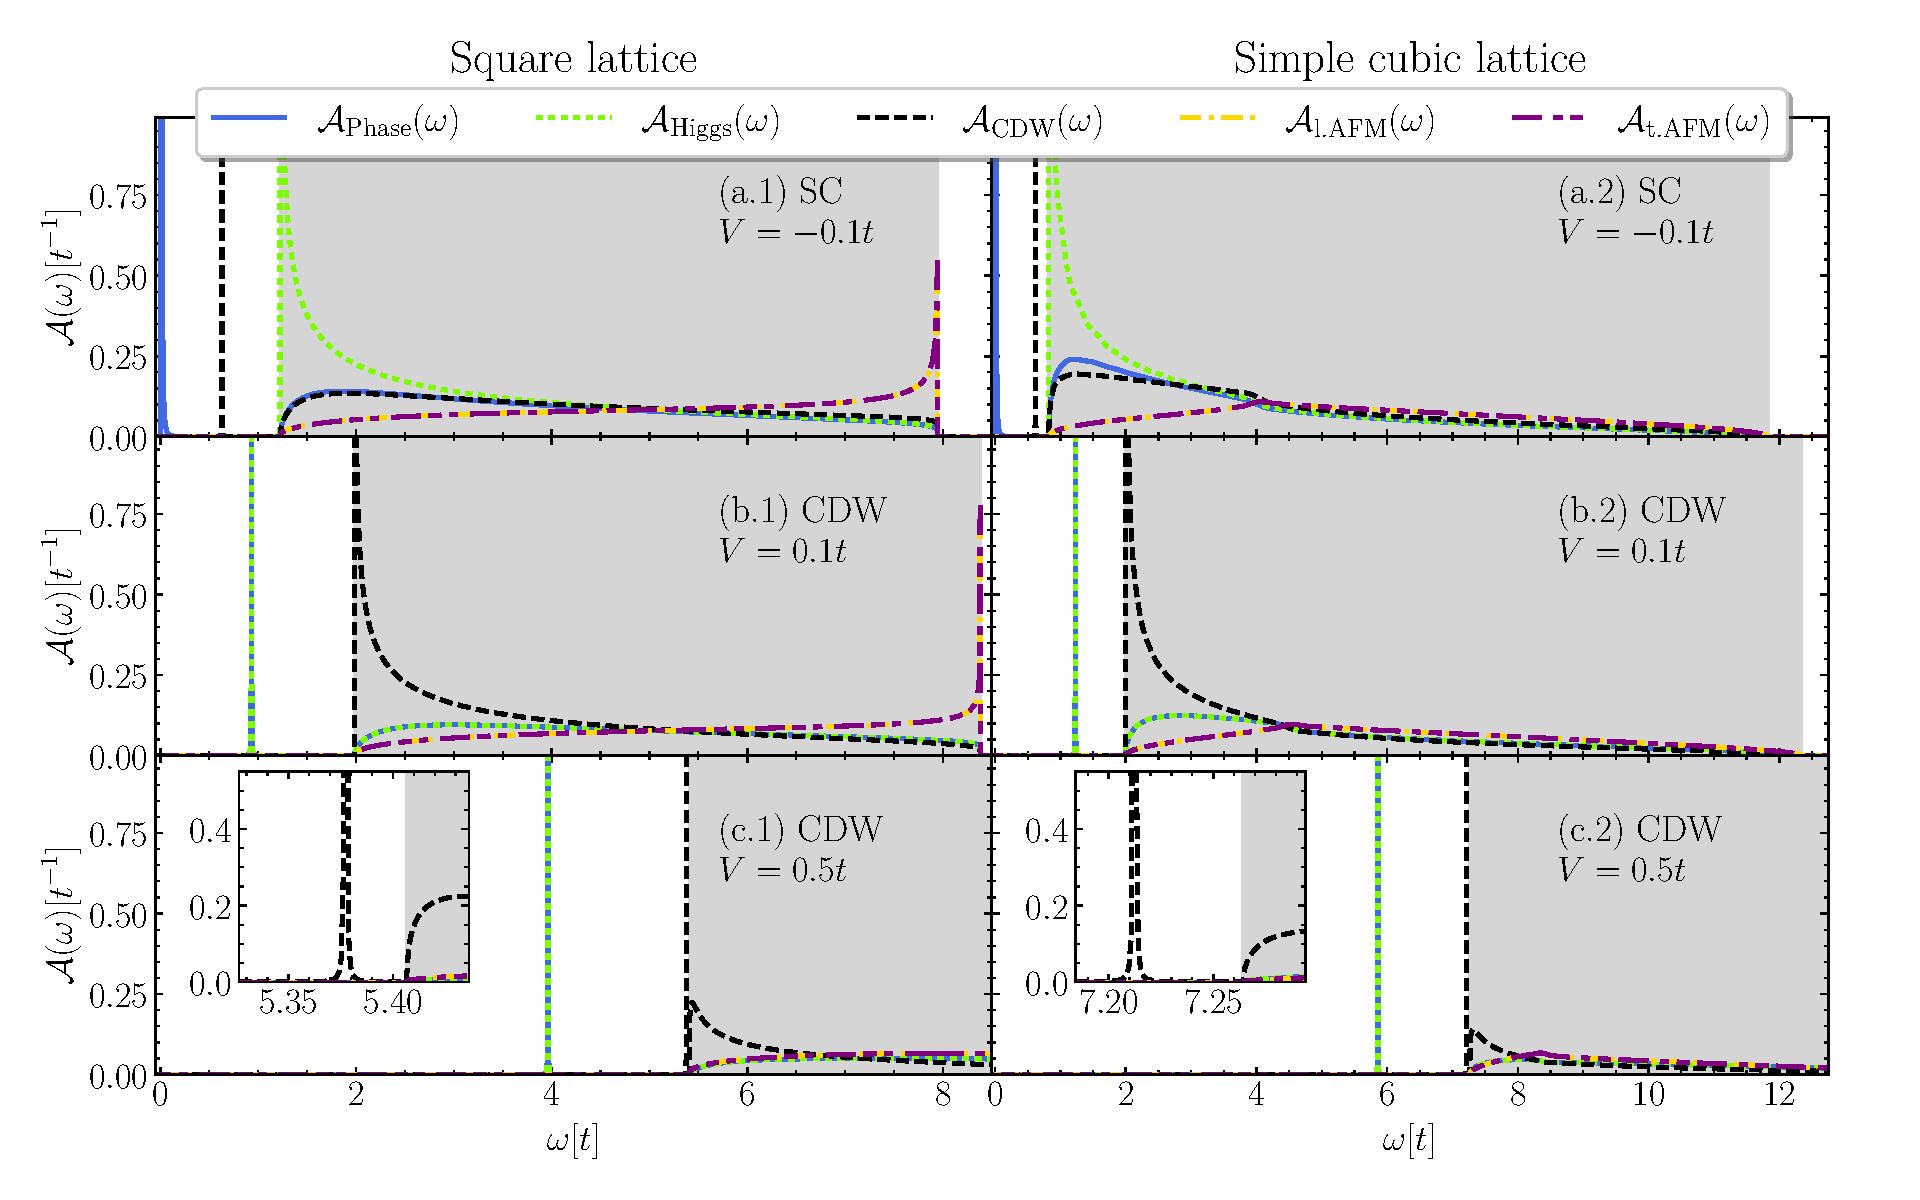
\includegraphics[width=.98\textwidth]{plots/resolvent_overview_SC_CDW.pdf}
    \caption{Spectral functions with respect to the operators listed in \eqref{eqn:resolvent_bases}.
    The left column shows the results for the square lattice while the right column shows the results for the simple cubic lattice.
    The left edge of each plot is at $-0.05$ rather than $0$ in order to improve the visibility of the phase peak.
    The shaded area marks the two-particle continuum.
    The panels (a), (b), and (c) show the spectral functions in the SC and CDW phases, respectively.}
    \label{fig:resolvent_overview_SC}
\end{figure*}

Let us first show and discuss the general form of the spectral functions in the SC and CDW phase and afterward, 
we will describe the behaviour of the occurring modes as the system approaches a phase transition.
\newline
The spectral functions corresponding to the individual operators in \eqref{eqn:resolvent_bases} are shown in \autoref{fig:resolvent_overview_SC}.
We chose $U=-2$ for the square lattice and $U=-2.5$ for the simple cubic lattice and $V=\pm0.1$ for both lattices.
\newline
There are a variety of different features. The difference between the two lattices is mostly quantitative in nature.
First and foremost, in the SC phase, there is a sharp peak located at $\omega=0$, only in the phase spectral function,
and another peak, only in the amplitude spectral function, located at $\omega=2\Delta_\text{SC}$.
We identify them with the well-known Leggett and Higgs modes in superconductors.
In the CDW phase, both of these spectral functions become identical and form a sharp peak below the two-particle continuum.
\newline
The CDW spectral function shows a peak below the continuum only in the SC phase, while having another peak at $\omega=2\Delta$ in the CDW phase.
The AFM spectral function is restricted to the continuum for both phases and both lattices.
For the square lattice, however, there is a peak located at the upper edge of the two-particle continuum.

To further classify the aforementioned peak that lie outside the two-particle continuum,
we turn towards the real part of the Green's function.
We plot it in close proximity to the peaks with a double logarithmic scale and fit the result linearly to obtain.

It is related to the imaginary part by the Kramers-Kronig relations.

\subsection{AFM-CDW transition}

\begin{figure*}
    \centering
    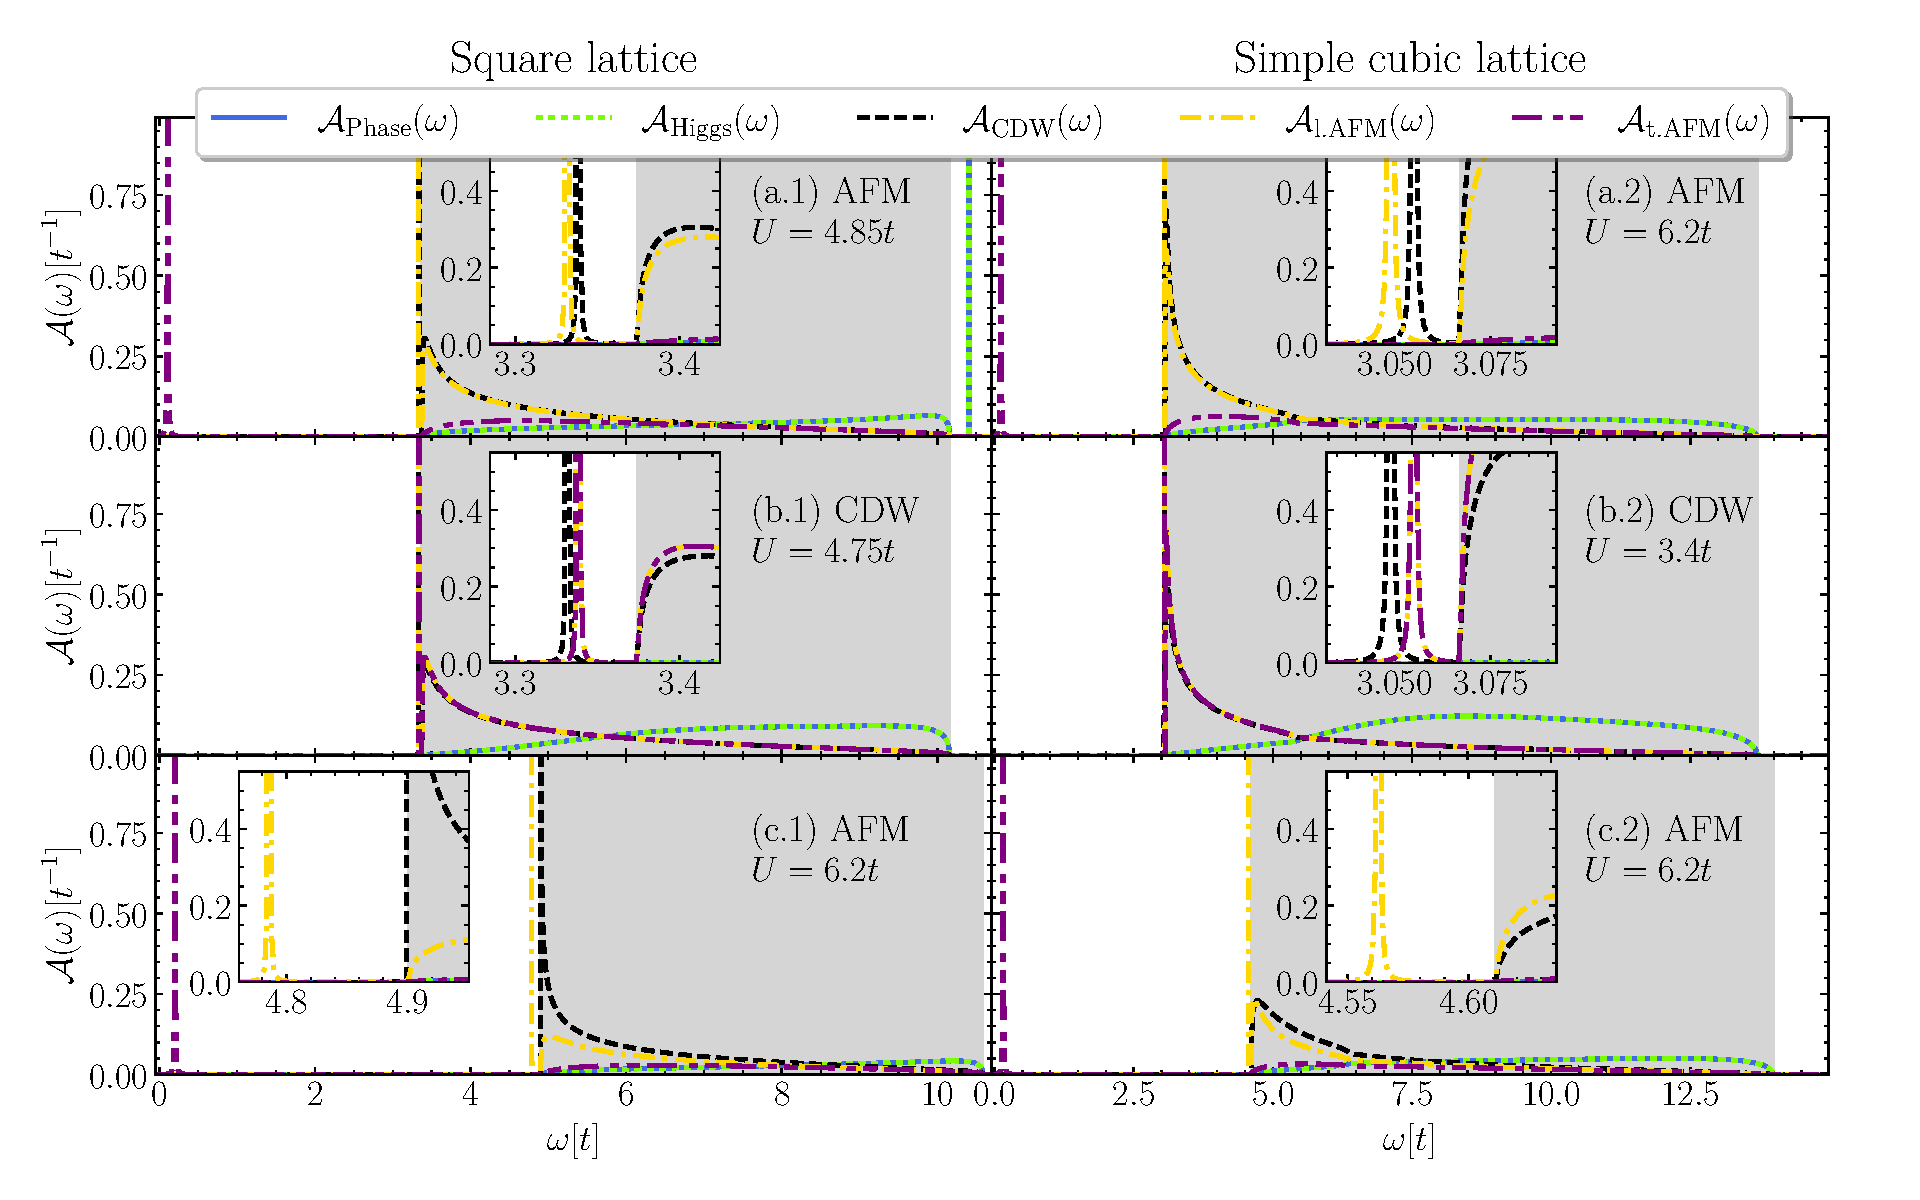
\includegraphics[width=.98\textwidth]{plots/resolvent_overview_AFM_CDW.pdf}
    \caption{Spectral functions with respect to the operators listed in \eqref{eqn:resolvent_bases}.
    The left column shows the results for the square lattice while the right column shows the results for the simple cubic lattice.
    %The left edge of the plots is at $-0.05$ rather than $0$ in order to improve the visibility of the phase peak.
    The shaded area marks the two-particle continuum.
    The panels (a) and (b) show the spectral functions in the CDW and AFM phases, respectively.}
    \label{fig:resolvent_overview_AFM}
\end{figure*}

Similar to the previous section, we will first show the general form of the spectral functions with respect to the operators \eqref{eqn:resolvent_bases}.
They are depicted in \autoref{fig:resolvent_overview_AFM}, choosing $V=1$ for the square lattice and $V=0.75$ for the simple cubic lattice.
For the CDW phase (panel a) we chose $U=ZV + 0.1$ and for the AFM phase (panel b) $V=ZV - 0.1$.


%%%%%%%%%%%%%%%%%%%%%%%%%%%%%%%%%%%%%%%%%%%%%%%%%%%%%%%%%%%%%%%%%%%%%%%%%%%%%%%%%%%%%%%%%%%%%%%%%%%%%%%%%%%%%%%%%%%%%
%%%%%%%%%%%%%%%%%%%%%%%%%%%%%%%%%%%%%%%%%%%%%%%%%%%%%%%%%%%%%%%%%%%%%%%%%%%%%%%%%%%%%%%%%%%%%%%%%%%%%%%%%%%%%%%%%%%%%
%%%%%                                                Conclusion                                                 %%%%%
%%%%%%%%%%%%%%%%%%%%%%%%%%%%%%%%%%%%%%%%%%%%%%%%%%%%%%%%%%%%%%%%%%%%%%%%%%%%%%%%%%%%%%%%%%%%%%%%%%%%%%%%%%%%%%%%%%%%%
%%%%%%%%%%%%%%%%%%%%%%%%%%%%%%%%%%%%%%%%%%%%%%%%%%%%%%%%%%%%%%%%%%%%%%%%%%%%%%%%%%%%%%%%%%%%%%%%%%%%%%%%%%%%%%%%%%%%%

\section{Conclusion}\label{sec:conclusion}

...


%==============================================================================
% Acknowledgments 
%==============================================================================
\begin{acknowledgments} 
    ....
\end{acknowledgments}

\bibliography{sn-bibliography}
%\bibliography{../../A_bibinput/liter10.bib}
		
\end{document}
